\documentclass[18 pt]{beamer}
\usetheme{Madrid}
% \usefonttheme{professionalfonts}
\usefonttheme{structurebold}
\usecolortheme{rose}
\setbeamerfont{title}{size=\LARGE, series=\bfseries}
% \setbeamerfont{subtitle}{size=\large}
% \setbeamerfont{author}{size=\large}
% \setbeamerfont{date}{size=\large}
% \setbeamerfont{frametitle}{size=\Large, series=\bfseries}
% \setbeamerfont{framesubtitle}{size=\large}
% \setbeamerfont{normal text}{size=\huge}
\usepackage{enumitem}
\setlist[enumerate]{label=\indent\indent, leftmargin=*,itemsep=30pt}
\setbeamerfont{enumerate item}{size=\LARGE}

\usepackage{amsmath}
\usepackage{amssymb}
\usepackage{listings}
\usepackage{booktabs}
\usepackage{multirow}
\usepackage{multirow}
\usepackage{lmodern}
\usepackage{xcolor}
\usepackage{float}
\lstset{
  language=Python,  %代码语言使用的是matlab
  % frame=shadowbox, %把代码用带有阴影的框圈起来
  rulesepcolor=\color{red!20!green!20!blue!20},%代码块边框为淡青色
  keywordstyle=\color{blue!90}\bfseries, %代码关键字的颜色为蓝色,粗体
  commentstyle=\color{red!10!green!70}\textit,    % 设置代码注释的颜色
  basicstyle=\footnotesize,
  showstringspaces=true,%不显示代码字符串中间的空格标记
  % numbers=left, % 显示行号
  % numberstyle=8pt,    % 行号字体
  % numberstyle=\color{green},
  stringstyle=\rmfamily\slshape\color[RGB]{128,0,0}, % 代码字符串的特殊格式
  breaklines=true, %对过长的代码自动换行
  extendedchars=false,  %解决代码跨页时,章节标题,页眉等汉字不显示的问题
  escapeinside=``,%代码中出现中文必须加上,否则报错
  texcl=true}

\lstset{breaklines}%自动将长的代码行换行排版

\lstset{extendedchars=false}%解决代码跨页时,章节标题,页眉等汉字不显示的问题

\usepackage{textcomp}
% \usepackage[margin=1in]{geometry}
\usepackage{pythonhighlight}
% \usepackage{minted}
\usepackage[backend=bibtex]{biblatex}
%\usepackage[style=authortitle,backend=biber]{biblatex}
\addbibresource{ResearchRabbit_Export_2022_10_20.bib}

\usepackage{algorithm}
\usepackage{algorithmic}
\renewcommand{\algorithmicrequire}{\textbf{Input:}}
\renewcommand{\algorithmicensure}{\textbf{Output:}}

\AtBeginSection[]{
  \begin{frame}
  \frametitle{Outline}
  \tableofcontents[currentsection]
  \end{frame}
}
\setbeamertemplate{section in toc}{\inserttocsectionnumber.~\inserttocsection}
\setbeamertemplate{subsection in toc}[ball unnumbered]
\setbeamertemplate{subsubsection in toc}[square unnumbered]


\title{Trapped-ion Quantum Computation introduction}
\author[Gcc]{Dingchao Gao}
\institute[ISCAS]{Institute of Software Chinese Academy of Sciences}

\setbeamertemplate{footline}[frame number]
\begin{document}

\begin{frame}[plain]
  \titlepage
\end{frame}
\section{Background}
\subsection{Quantum numbers}
\begin{frame}
  \frametitle{Quantum numbers}
  \begin{enumerate}
    \item Principal Quantum Number \(n=1,2,3,\dots\)
    \item Azimuthal Quantum Number \(l=0,\dots,(n-1)\)
    \item Magnetic Quantum Number \(m_l=-l,\dots,l\)
    \item Electron Spin Quantum Number \(m_s=-\frac{1}{2},+\frac{1}{2}\)
  \end{enumerate}
\end{frame}
\begin{frame}
  \frametitle{Quantum numbers}
  \begin{figure}
    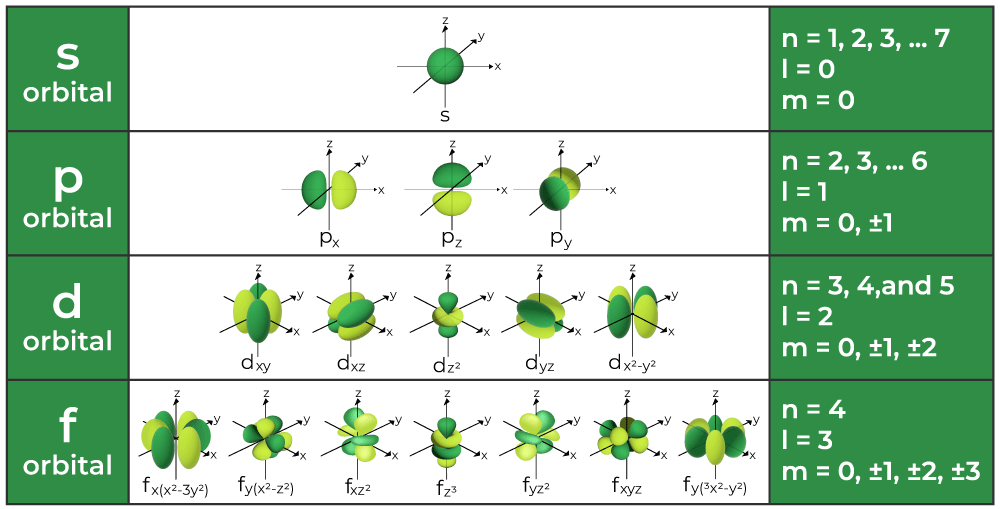
\includegraphics[width=.8\linewidth]{QuantumNumbers.png}
    \caption{copy from \footcite{https://www.geeksforgeeks.org/quantum-numbers/bibid}}
  \end{figure}
\end{frame}
\begin{frame}
  \begin{enumerate}
    \item Pauli exclusion principle
    \item Aufbau principle
    \begin{figure}
      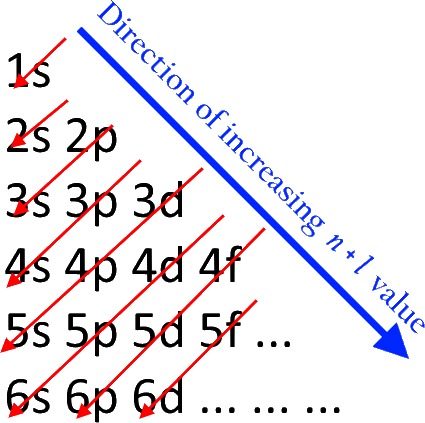
\includegraphics[width=.3\linewidth]{Aufbau_Principle.png}
      \caption{copy from \footcite{https://en.wikipedia.org/wiki/Aufbau_principle}}
    \end{figure}
  \end{enumerate}
\end{frame}
\begin{frame}
  \frametitle{Examples on Quantum numbers}
  For Rubidium has the atomic number, Z = 37.\\
  Electronic Configuration of Rubidium,\(1s^22s^22p^63s^23p^63d^{10}4s^24p^65s^1\)
  \begin{enumerate}
    \item Principal Quantum Number \(n = 5\)
    \item Azimuthal Quantum Number \(l = 0\)
    \item Magnetic Quantum Number \(m_l = 0\)
    \item Spin Quantum Number \(m_s = +1/2\)
  \end{enumerate}
\end{frame}
\begin{frame}
  \frametitle{splitting methods}
  \begin{figure}
    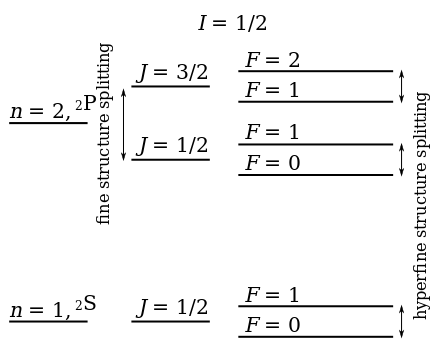
\includegraphics[width=.6\linewidth]{440px-Fine_hyperfine_levels.svg.png}
    \caption{copy from \footcite{https://en.wikipedia.org/wiki/Hyperfine_structure}}
  \end{figure}
\end{frame}
\subsection{Cooling techniques}
\begin{frame}
  \frametitle{doppler cooling}
  \begin{figure}
    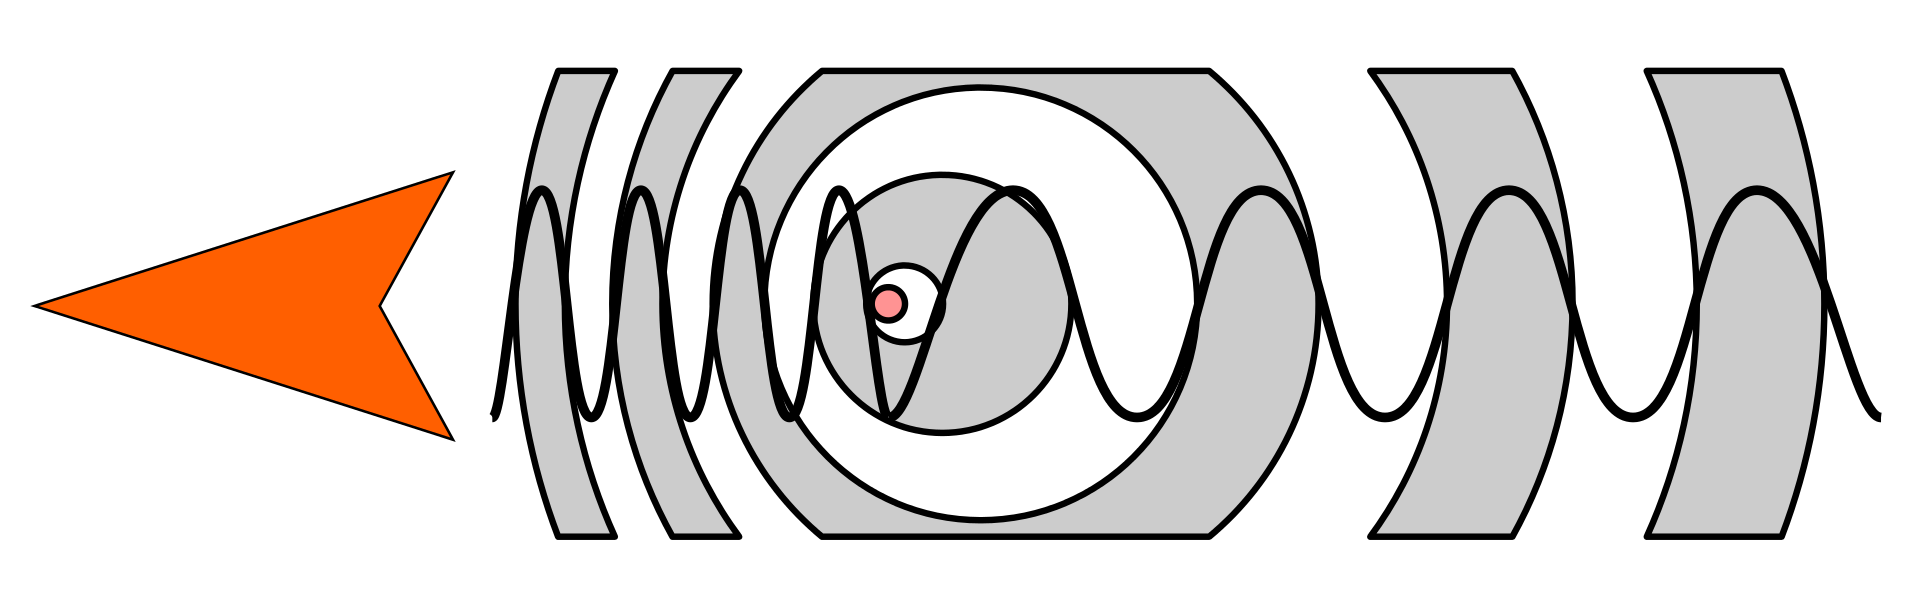
\includegraphics[width=.8\textwidth]{1920px-Doppler_effect_diagrammatic.svg.png}
    \caption{copy from \footcite{https://en.wikipedia.org/wiki/Doppler_cooling}}
  \end{figure}
\end{frame}
\begin{frame}
  \frametitle{Resolved sideband cooling}
  \begin{figure}
    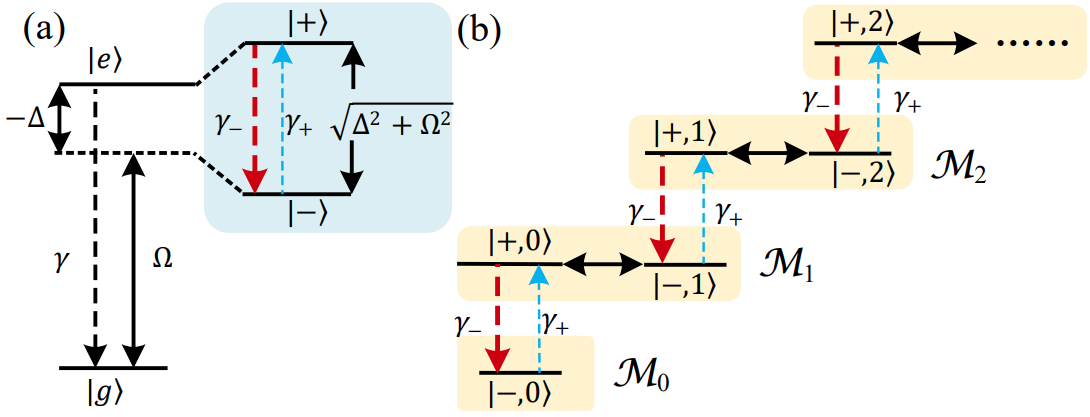
\includegraphics[width= .4\textwidth]{sideband.png}
    \caption{copy from \footcite{https://arxiv.org/pdf/2211.08896.pdf}}
  \end{figure}
\end{frame}

\subsection{Ion trapping methods}
\begin{frame}
  \frametitle{paul traps}
  % figure here
\end{frame}
\begin{frame}
  \frametitle{penning traps}
  %  figure here
\end{frame}
\section{Qubit types}
\begin{frame}{}
  \frametitle{Qubit Type Comparison}
  \begin{figure}
    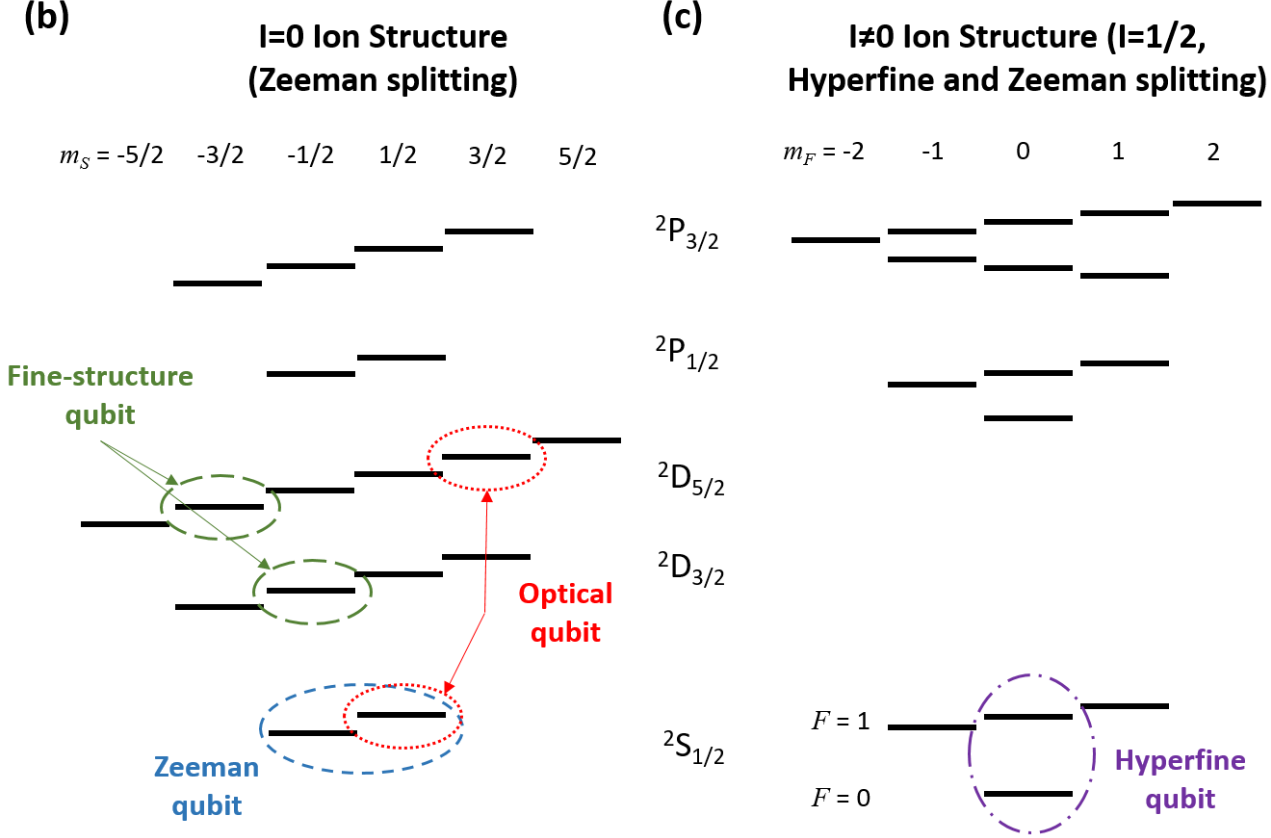
\includegraphics{qubit.png}
    \caption{copy from \footcite{https://arxiv.org/abs/1904.04178}}
  \end{figure}
\end{frame}
\begin{frame}
  \frametitle{key factors in coherence time}
  \begin{enumerate}
    \item Abbe diffraction limit \(d = \frac{\lambda}{2n\sin\theta}=\frac{\lambda}{2NA}\)
    \item Spontaneous emission rate
    \item Magnetic field fluctuations
    \item Laser technical noise
  \end{enumerate}
\end{frame}
\section{Qubit control}
\subsection{signal qubit gates}
\begin{frame}
  \frametitle{signal qubit gates}
  % optical transitions (for optical qubits), Raman transitions (for hyperfine/Zeeman qubits), or microwaves.
  \begin{figure}
    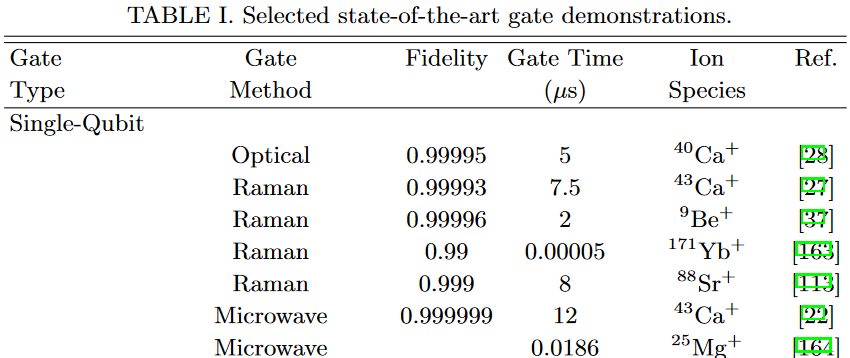
\includegraphics[width=.8\textwidth]{singal-gate.png}
    \caption{copy from \footcite{https://arxiv.org/abs/1904.04178}}
  \end{figure}
\end{frame}
\subsection{multi qubit gates}
\begin{frame}
  \frametitle{Two Qubit Gates}
  \begin{enumerate}
    \item Cirac-Zoller
    \item Mølmer-Sørensen
  \end{enumerate}
\end{frame}
\begin{frame}
  \frametitle{challenges for gates}
  \begin{enumerate}
    \item Crosstalk
    \item Laser frequency/amplitude stability
    \item Motional heating (two qubit gates)
    \item \(\dots\)
  \end{enumerate}
\end{frame}
\subsection{measurement}
\section{Scaling}

\end{document}